%!TeX spellcheck = en_US
\setlength{\pdfpagewidth}{210mm}
\setlength{\pdfpageheight}{297mm}
\documentclass[journal,transmag]{IEEEtran}
\usepackage{amsmath}
\usepackage{subfigure}
\hyphenation{op-tical net-works semi-conduc-tor}
\usepackage{hyperref,color,breqn,multirow}
\usepackage[top=0.7in, left=0.65in]{geometry}
\usepackage{graphicx}
\setlength{\textwidth}{7.2in}
\setlength{\textheight}{9.6in}

\begin{document}
\title{An Improved Domain Decomposition with Relaxation Method Used for Dynamic Simulation of Electromagnetic Devices}


\author{\IEEEauthorblockN{Wenying Yang\IEEEauthorrefmark{1},
		Zilan Qiu\IEEEauthorrefmark{1}, 
		Fei Peng\IEEEauthorrefmark{1} and
		Guofu Zhai\IEEEauthorrefmark{1}}
\IEEEauthorblockA{\IEEEauthorrefmark{1}School of Electrical Engineering and Automation, Harbin Institute of Technology, Harbin, 150001 China}}	


\IEEEtitleabstractindextext{%
\begin{abstract}
Finite element method (FEM) is necessary to analyze the dynamic characteristics of electromagnetic mechanisms. Parallel technology makes the computation of FEM more effective, such as domain decomposition (DD) method. In this paper, a new finite element solution technique called nodal domain decomposition with relaxation (NDDR) is used to solve the dynamic characteristics of the electromagnetic device. This method can improve the parallelism to accelerate the dynamic characteristic solving. To greatly improve the solving efficiency of NDDR method, we introduce Robin-type transmission condition to it. 
%有限元方法是分析电磁机构动态特性的必要手段,通过区域分解实现并行化能有效提高有限元方法的求解速度。本文采用nodal domain decompositon with relaxation的有限元并行求解技术来解算电磁机构的动态特性,并且针对原本NDDR方法中存在的计算效率不足的问题提出改善措施。(什么措施??)(对比验证怎么加上??)
\end{abstract}

\begin{IEEEkeywords}
Domain decompositon (DD), Dynamic analysis, Electromagnetic apparatus, Finite element method (FEM), Parallel algorithm
\end{IEEEkeywords}}

\maketitle
\thispagestyle{empty}
\pagestyle{empty} 

\section{Introduction}
\IEEEPARstart{I}{N} electromagnetic apparatus, electromagnetic devices are often used to drive contact separating or other load work. Although the static simulation is usually performed to judge the characteristic of the electromagnetic device in engineering, it is the dynamic characteristic that determines the movement process of the electromagnetic device. Therefore, analysis of dynamic characteristics plays an important part in the design of electromagnetic apparatus \cite{IEEEhowto:Wang}.
%在开关电器中,常用电磁铁作为驱动元件来带动触头分合和其他负载做功。尽管电磁机构的静态过程常用于电磁机构的分析,但是电磁机构的动态特性更能正确反映其工作特性,因此动态特性的分析对于开关电器的设计至关重要。\cite{IEEEhowto:Wang}

In the computation of the dynamic characteristic, the electromagnetic field distribution is necessary to be calculated when the armature moves at different positions \cite{IEEEhowto:You}. The finite element method (FEM) is widely used to calculate the electromagnetic field distribution. Many scholars have studied the acceleration of FEM process in electromagnetic field. Recently, some scholars have proposed a new nodal domain decomposition with relaxation method (NDDR) for electromagnetic field parallel calculation, which has achieved excellent acceleration effect  \cite{IEEEhowto:Liu}.
%在动态特性的计算过程中,需要计算铁芯在不同位置处的磁场分布,以求解出磁场力,进而求解电磁机构的运动特性。\cite{IEEEhowto:You}计算磁场分布一般采用有限元方法,许多学者研究了有限元电磁场求解加速的方法。通过区域分解来实现并行计算,将求解任务分发给CPU的多个核或者是交给GPU求解,是电磁场有限元求解加速的一大趋势。\cite{IEEEhowto:Dziekonski}近期有学者提出了一种新的NDDR方法,用于电器产品的电磁场并行计算,取得了很好的加速效果。\cite{IEEEhowto:Liu}

The computation of dynamic characteristic always consumes a lot of computing resources, so it is necessary to find a way to accelerate the solving process. The NDDR method achieves a good acceleration effect in the calculation of the static electromagnetic field distribution, however, few scholars pay attention to its use in dynamic characteristic solving. What's more, it is believed that NDDR method's efficiency need to be further improved. In this paper, we apply the Robin type condition in the interface of two adjacent domains to improve the convergence speed of NDDR method, and apply this method to accelerate the solution of the dynamic characteristic. 
%电磁机构动态特性的计算量大,计算速度慢,因此提出一种加速电磁系统动态特性求解的方法至关重要,尽管NDDR方法在电磁机构的磁场分布计算中取得了很好的加速效果,但是并没有学者研究如何将其应用至动态特性的求解过程当中,且该方法本身的求解效率也可以进一步完善。所以在本文中,我们提出一种改良NDDR求解效率的方法,并且通过该方法来加速电磁机构动态特性的求解。

\section{Improved Nodal Domain Decomposition With Relaxation Method}
Both conventional domain decomposition (DD) method and NDDR method focus on accelerating the solution of FEM using parallel techniques. Conventional DD method is shown in Fig. \ref{fig:ddm}, the whole solution domain is decomposed into several subdomains and processed separately by different cores of CPU. The fewer nodes and elements that each core is required to process, the higher solution efficiency can obtain. Therefore, NDDR method proposes an extreme idea, which means only one node in a subdomain, as showed in Fig. \ref{fig:nddr}. In this way, the degree of parallelism is greatly increased. In the case where the number of cores is sufficient, each core only needs to solve one node unit, and the solving efficiency can be significantly improved.
%DD方法和NDDR方法都是通过并行化来加速求解有限元的方法。传统的区域分解方法如图\ref{nddr}(a)所示,通过区域分解,整个求解域被分解成数个子域,将子域分给CPU的多个核分别进行处理,通过灵活控制子域相交处的边界条件进行迭代求解。考虑到区域分解中,并行化程度越高,每个核需要处理的节点和单元数目越少,求解效率越高。所以在NDDR方法中,省略了传统的装配过程,将每一个节点视为一个单独的子域。这样的方式使得并行度极大的增加,在核的数目足够多的情况下,每一个核只需要求解一个节点单元,求解效率可以得到很大的提升。

\begin{figure}
	\centering
	\subfigure[Conventional DD method ]{
		\label{fig:ddm}
		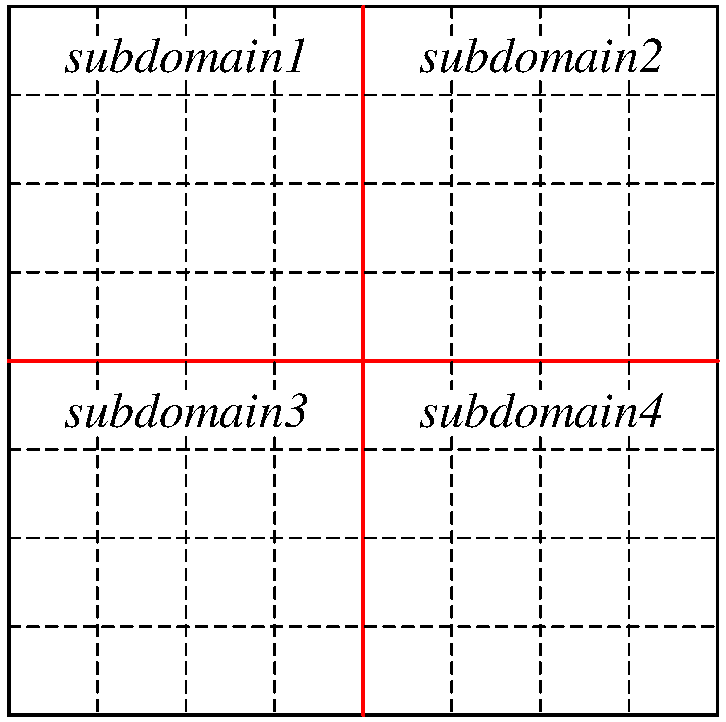
\includegraphics[width=0.4\linewidth]{ddm.pdf}}
	\subfigure[NDDR method]{
		\label{fig:nddr}
		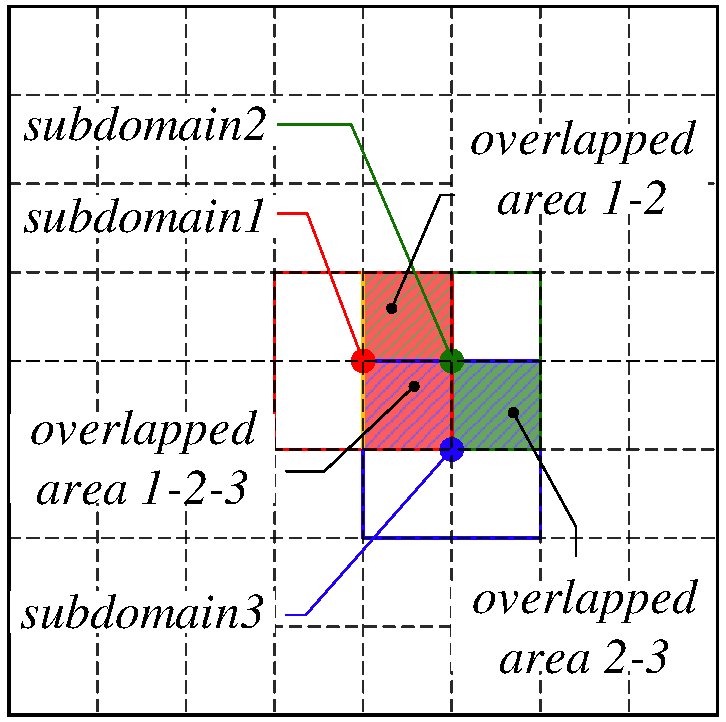
\includegraphics[width=0.4\linewidth]{nddr.pdf}}
	\caption{Comparation between conventional DD method and NDDR method}
\end{figure}
Although NDDR method has achieved good acceleration in static electromagnetic solving, its efficiency can still be improved. In the case study of NDDR method proposed by \cite{IEEEhowto:Liu}, thousands of GPU cores are used to solve the electromagnetic distribution, but the acceleration effect obtained is only tens of times. What's more, with the number of nodes increases, each core need to process multiple nodes, and the solution efficiency is further reduced.
%NDDR和能够取得良好加速效果的关键在于其高度的并行性,大大减小了每个核的求解压力,但是仍然存在可以改进的地方。在\cite{IEEEhowto:Liu}提出的NDDR方法的求解静态电磁场分布的实例当中,可以看到,尽管采用了几千个核进行求解,但是取得的加速效果仅有数十倍,而且随着节点数目的增加,有求解单元需要负担多个域的求解任务时,求解速度进一步降低。
%(这个方法应该怎么编??)

In conventional DD method, using Robin-type transmission condition  can obtain faster convergence speed than Dirichlet-type transmission condition \cite{IEEEhowto:Douglas}. Therefore, we introduce Robin-type transmission condition to NDDR method, to improve the solution efficiency of NDDR.
%考虑到区域分解法通常以Dirichlet条件作为界面传输条件,而Robin条件作为界面传输条件可以大大加快算法的收敛速度,为此我们在求解域的交界处引入Robin条件,以达到改进NDDR求解速度的目的。
\section{Dynamic Analysis With NDDR}
To solve the dynamic characteristic of an electromagnetic device, we need to calculate differential equations for electromagnetic field distribution. The solution of the electromagnetic field distribution is consistent with the solution of the static magnetic field. The differential equations of the electromagnetic field are solved by FEM. It can be described as follows:
%为了求解电磁系统的动态特性,我们需要求解电磁场分布和动态特性的微分方程。电磁场分布的求解和静磁场的求解方式一致,都是将电磁场的微分方程通过有限元法求解。磁场问题可由以下方程描述:
\begin{equation}
\left\{
\begin{aligned}
&{\nabla\cdot}A=B\\
&\nabla\cdot({\upsilon\nabla}A)=-J
\end{aligned}
\right.
\end{equation}
where $A$ is the magnetic filed potential vector, $B$ is the magnetic induction, $\upsilon$ is the magnetic permeability and $J$ is the current density. 

After each sub-network are discredited by Galerkin's method \cite{IEEEhowto:Rao}, a set of equations in the element can be obtained:
%其中,$A$是磁矢位,$B$是磁感应强度,$\upsilon$是磁导率,$J$是电流密度。通过伽辽金方法\cite{IEEEhowto:Rao}对每个分网后的单元进行离散后,可以得到单元内的一组方程
\begin{equation}
[S^e][A^e]=[F^e]
\end{equation}
where $[S^e]$ relates to the node coordinates in the element, $[A^e]$ represents magnetic filed potential vector of each node and $[F^e]$ relate sto the size of element and the current density in the element.
%$S$内的元素只与当前单元内的节点坐标相关,$A$表示各个节点内的磁矢位,$F$与电流密度和单元大小相关 (需要具体解释一下)

During the usual finite element solution process, each element needs to be assembled after element analysis. Then we need to solve a nonlinear large sparse symmetric positive definite (SPD) system. The finite element solution of the dynamic characteristic in this paper is achieved by improved NDDR method, which avoids the assembly process of the matrix and improves the efficiency of the solution through parallelization.
%在通常的有限元求解流程中,需要将每个单元分析后的系统进行装配,最终求解一个大型SPD系统。本文中动态特性的有限元求解通过NDDR方法实现,该方法省略了矩阵的装配过程,并且通过并行化提高了求解效率。

In the dynamic characteristic electromagnetic field solving process, the position of the armature in each time step is different, and the whole domain needs to be re-meshed and re-solved. Considering that the electromagnetic field at the same position does not change much, we can use the final value in the previous solution at the same position as the initial value of the next solution to achieve the iterative acceleration effect.
%动态特性电磁场求解过程中,每一个时间步的铁芯位置不同,需要进行重新分网和求解。考虑到相同位置处的磁场变化不大,所以我们将处在同一位置的前一次求解中最终值作为下一次求解的初始值,以此来达到迭代加速的效果。
%(我觉得这一部分可以大改,但是怎么改?)

The differential equations of dynamic characteristics include circuit equations and motion equations:
%动态特性的微分方程包括电路方程和运动方程。
\begin{equation}
\left\{ 
\begin{aligned}
&u = iR + \frac{{d\psi }}{{dt}}\\
&m\frac{{{d^2}x}}{{d{t^2}}} = F - {F_f}
\end{aligned} 
\right.
\label{dynamic}
\end{equation}
where $u$, $i$, $R$ represent the voltage, current and resistance of the coil, $\psi$ is the flux linkage, $m$ is the mass of armature, $F$ is the electromagnetic force and $F_f$ is the load reaction force.
%式中,$u$,$i$,$R$分别为线圈的电压,电流和电阻,$\psi$为磁链大小,$m$为衔铁质量,$F$为电磁吸力,$F_f$为负载反作用力。

To simplify the solving process, converting \eqref{dynamic} to the form of the first derivative equations as shown:
%为了方便求解,将\eqref{dynamic}转换成一阶导数方程组的形式后如下所示:
\begin{equation}
\left\{
\begin{aligned}
&\frac{{di}}{{dt}} = \frac{{u - iR}}{L} - \frac{i}{L}\frac{{dL}}{{dt}}\\
&\frac{{dv}}{{dt}} = \frac{1}{m}(F - {F_f})\\
&\frac{{dx}}{{dt}} = v
\end{aligned}
\right.
\end{equation}
where $L$ is the magnetic system inductance.
%其中,$L$为磁系统电感。

In this paper, we use the weak coupling method to solve the dynamic characteristics of the electromagnetic system. The solving process is shown in Fig. \ref{fig:flowchart}. The difference equation in this process can be solved by fourth-order Runge-Kutta method.
%在本文中,我们采用弱耦合的方式求解电磁系统的动态特性。求解流程图如图\ref{fig:flowchart}所示。该流程中差分方程采用四阶龙格-库塔方法求解。
\begin{figure}
	\centering
	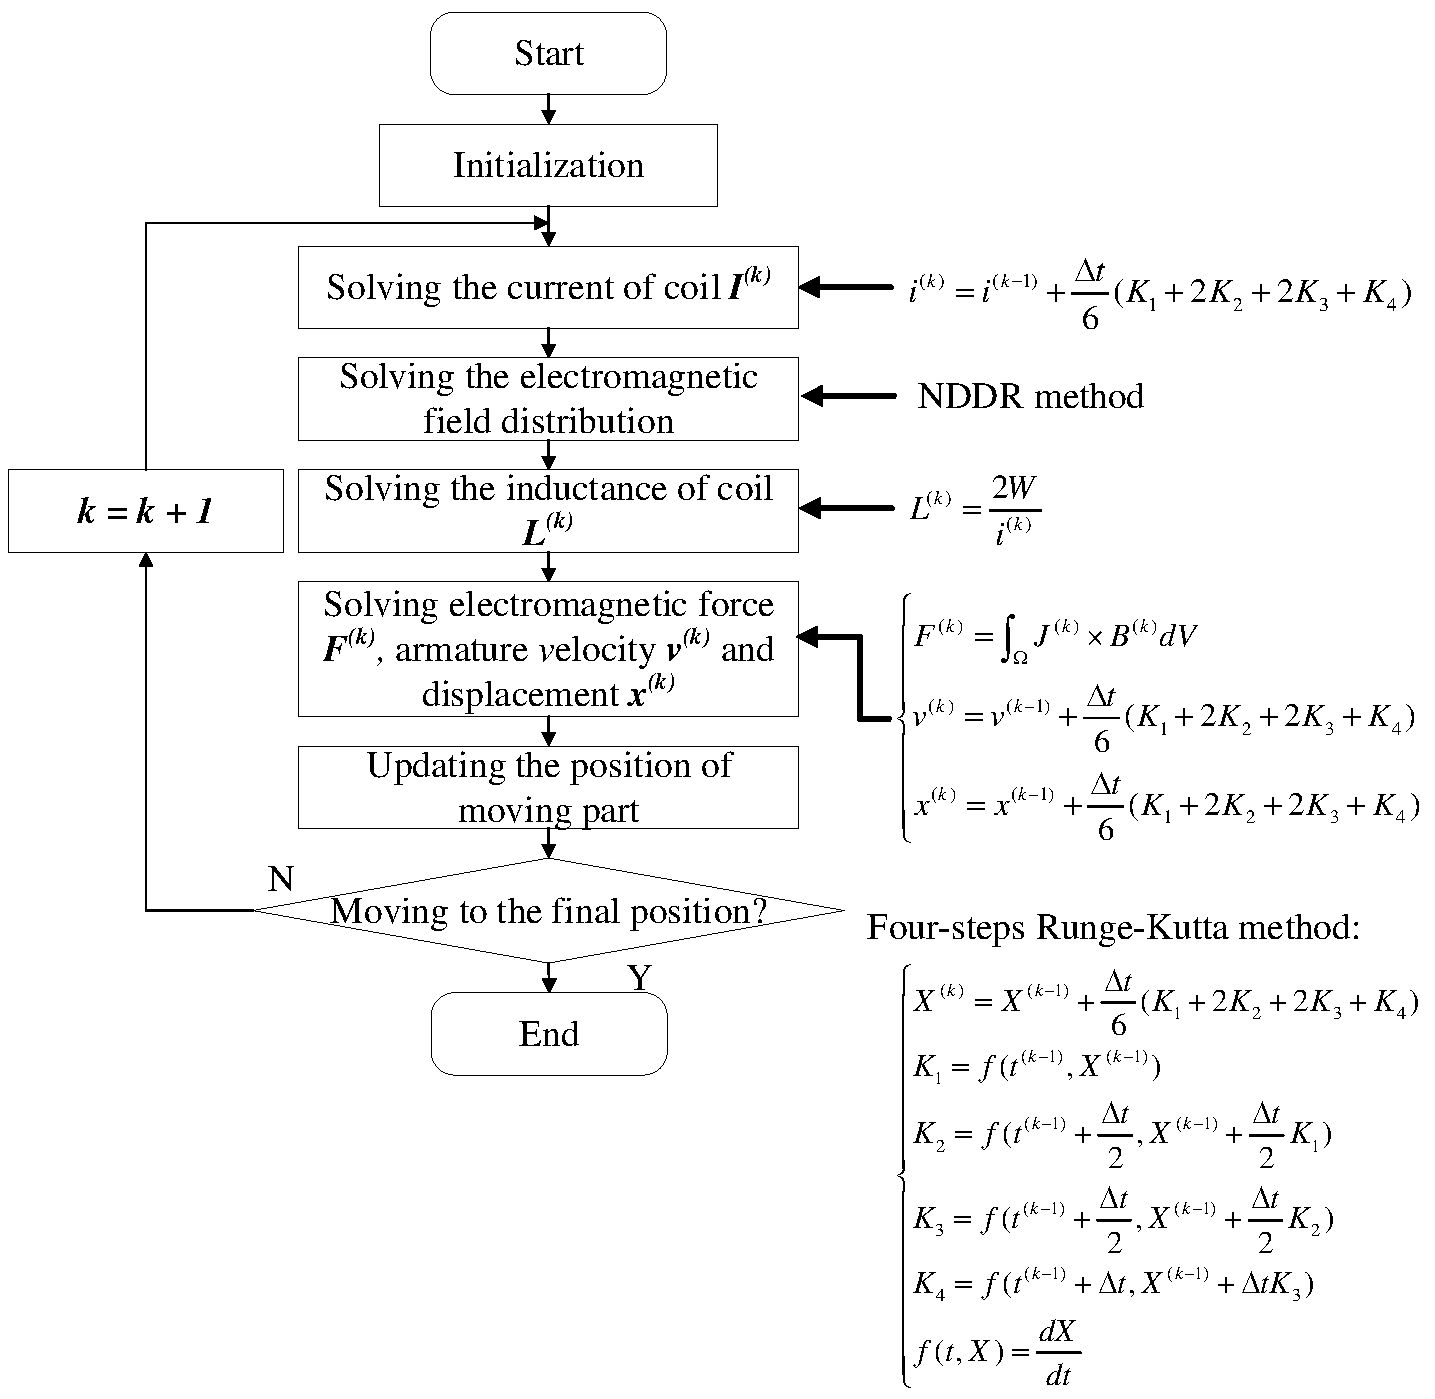
\includegraphics[width=1.0\linewidth]{flowchart.pdf}
	\caption{Dynamic solving process with NDDR}
	\label{fig:flowchart}
\end{figure}

\section{Case Study}
In order to verify that the NDDR method can accelerate the solution of electromagnetic field dynamics, this paper uses a dynamic model of the solenoid contactor to calculate, and finally compares with the solution efficiency and solution accuracy of COMSOL. The model that needs to be solved is shown in Fig. \ref{fig:simple2}.
%为了验证NDDR方法确实能够加速电磁场动态特性的求解,本文使用螺管式接触器的动态模型进行求解验证,并且最终与COMSOL的求解效率和求解精度进行对比。需要求解的模型如图\ref{fig:simple2}所示。
\begin{figure}
	\centering
	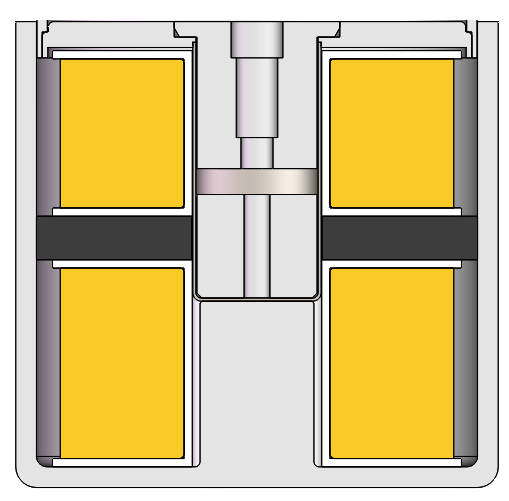
\includegraphics[width=0.4\linewidth]{simple2}
	\caption{The model of solenoid contactor}
	\label{fig:simple2}
\end{figure}


\begin{thebibliography}{1}
\bibitem{IEEEhowto:Wang}
S.- Wang, T. Miyanao, and M. Hubbard, “Electromagnetic field analysis and dynamic simulation of a two-valve solenoid actuator,” IEEE Transactions on Magnetics, vol. 29, no. 2, pp. 1741–1746, Mar. 1993.

\bibitem{IEEEhowto:You}
Y. Jiaxin, L. Huimin, M. Guangcheng, C. Shuqing, and C. Zhaowen, “Research on the dynamic calculation model for a dc solenoid electromagnetic contactor and its contact characteristics in break process,” in 2015 IEEE 61st Holm Conference on Electrical Contacts (Holm), 2015, pp. 191–194.
	
%\bibitem{IEEEhowto:Dziekonski}
%A. Dziekonski, A. Lamecki, and M. Mrozowski, “GPU-accelerated finite element method,” in 2016 IEEE MTT-S International Conference on Numerical Electromagnetic and Multiphysics Modeling and Optimization (NEMO), 2016, pp. 1–2.

\bibitem{IEEEhowto:Liu}
P. Liu and V. Dinavahi,``Matrix-Free Nodal Domain Decomposition With Relaxation For Massively Parallel Finite-Element Computation of EM Apparatus,” IEEE Transactions on Magnetics, vol. 54, no. 9, pp. 1–7, Sep. 2018.

\bibitem{IEEEhowto:Douglas}
J. Douglas and C.-S. Huang, “An accelerated domain decomposition procedure based on robin transmission conditions,” BIT Numerical Mathematics, vol. 37, no. 3, pp. 678–686, 1997.

\bibitem{IEEEhowto:Rao}
Rao, S. S . "The Finite Element Method in Engineering," Pergamon Press, 1982, pp. 194-198.

\end{thebibliography}

\end{document}
